\documentclass[10pt, onecolumn, draftclsnofoot, letterpaper, compsoc]{IEEEtran}

\usepackage{graphicx}
\usepackage{amssymb}
\usepackage{amsmath}
\usepackage{amsthm}
\usepackage{alltt}
%\usepackage{float}
\usepackage{color}
\usepackage{url}
\usepackage{minted}

\graphicspath{ {images/} }

\renewcommand*\contentsname{Table of Contents} % Rename ToC

% Temp title and author
\title{Midterm Progress Report}
\author{Totality AweSun \\
		Bret~Lorimore, Jacob~Fenger, George~Harder \\
		\textit{\today \\
		CS 462 - Winter 2017}}

\begin{document}

\maketitle

\begin{abstract}
This document describes the current state of the \textit{North American Solar Eclipse 2017}
senior capstone project. The document gives a brief overview of the project and its components,
describes the current state of the project, describes problems that have been
encountered throughout the term, shows some of the code that has been produced thus far, gives
a week-by-week outline of progress throughout the term, and reflects over the term in the
retrospectives section at the end.
\end{abstract}

\newpage

\tableofcontents

\newpage

%%%%%%%%%%%%%%%%%%%%%%%%
%   Project Overview   %
%%%%%%%%%%%%%%%%%%%%%%%%
\section{Project Overview}

The North American Solar Eclipse 2017 Senior Capstone project is partnered
with Google to build a set of applications that will assist the development of
the Eclipse Megamovie Project. The overall project has been broken down into
three components: the eclipse image processor, the image processor manager, and
the solar eclipse simulator. Each will be individually outlined in the sections
below.

\subsection{Image Processor}

The image processor’s primary activity is to quickly and consistently identify
images of an eclipse at totality. The Eclipse Megamovie project will be
collecting thousands of images from photographers around the country, and the
image processor needs to identify the images of the eclipse at totality so that
these can then be stitched into a timelapse movie. In order to make the
stitching as easy as possible for the Eclipse Megamovie team, the image
processor will add metadata to each processed image that includes spatial
information about where the image was taken along the path of totality and
temporal information about how far into totality the eclipse is.


The purpose of the Image Processor is not to process many images as quickly as
possible. Instead, our goal is to be able to consistently and accurately process
a single image at a time. As such, the image processor will fit into the larger
project as an executable file that is called by the Image Processor Manager.
This allows us to focus the image processor solely on a single goal, and leave
parallelization and deployment to a different piece of the project.

\subsection{Image Processor Manager}

The image processor manager will be a Python application responsible for managing the image processor
application. This includes collecting images from Google Cloud for the image processor to process,
invoking the image processor with these images as input, and collecting the output of the image
processor and uploading it to Google Cloud. The image processor and image processor manager will be
deployed together in a single docker container to Google Container Engine Clusters (of VMs). \\

An important role of the image processor manager is that it will be responsible for ensuring that
the compute resources on the host VMs are as saturated as possible. This means invoking multiple
image processor processes concurrently, while at the same time downloading the next images to be
processed and uploading the already processed images. The image processor manager will achieve
this parallelism through process based concurrency in Python, as in Python, thread based concurrency
is throttled by the global interpreter lock (GIL). We chose to use Python for this application as it
will be much simpler to write in Python and we can sidestep any concurrency issues by using process
based parallelism as mentioned above. \\

\subsection{Eclipse Simulator}

The eclipse simulator will be an independent JavaScript module that can easily
be added to the existing Eclipse Megamovie webpage. This simulator will allow
users to “preview” the eclipse. It will be a 2D depiction of what the solar
eclipse in 2017 could look like given a certain location. Users will be able
to interact with a time slider that will simulate the eclipse in a time
window spanning from 12 hours before the eclipse to 12 hours after it.

To help with the eclipse ephemeris computations, we will be using an external
JavaScript library called MeeusJs. For the front end view for the simulator,
we will be utilizing HTML5 SVG. We plan to implement a model-view-controller
architecture for controlling the states of each component as well as handling
the interactions. This architecture was chosen due to the ability to easily
exchange a component without altering the whole design of the system. For
example, if one wanted to create a whole new front end for the simulator,
they would not need to rewrite the model or controller component of the system.
They would simply need to ensure that the new view component can handle the
interactions with the controller module.


%%%%%%%%%%%%%%%%%%%%%%%%
%   Current Status     %
%%%%%%%%%%%%%%%%%%%%%%%%
\section{Current Status of the Project}

As a whole this project has moved from the pre-planning stages into the earliest
development phase. The image processor and the image processor manager are both
fully designed, while the eclipse simulator is farther along and has some existing proof of
concept code.

When this project was being planned,
the Image Processor was the main thrust of the project and the simulator was, in
our minds, a secondary objective that could be completed quickly. However, the
emphasis has shifted toward producing an extremely polished visualization of the
eclipse that will be included on the eclipsemega.movie site. This shift in
priorities as well as the delays with code becoming open-sourced has placed this
piece of the project on the back burner for the time being.

\subsection{Image Processor}

Development of the Image Processor is currently on hold for a couple of reasons.
First, the image processor relies on existing code from our project sponsor that
needs to be open-sourced before we can work with it. Our project sponsor has
been working on getting this code to us, however this process relies on approval
from several levels on management at Google and is a slow moving process. Based
on conversations with our sponsor we do not expect this code to become available
until the end of February or beginning of March. Secondly and as mentioned above,
there has been somewhat a shift in priorities for our sponsor.

\subsection{Image Processor Manager}

The image processor manager is currently on hold for the same reasons as the image processor,
outlined above.

\subsection{Eclipse Simulator}

We currently have a working eclipse simulator that meets the specs outlined in
our requirements document. This includes allowing users to simulate the eclipse
at locations across the United States by entering their location either via searchbar
of by selecting it on a map. This basic functionality was completed several weeks
ago, however we have been working on tuning and adding additional features after
presenting the initial MVP to our client.

Two new features that were requested are a zoom mode, allowing users to view a
close-up simulation of the eclipse, and a "play" feature, that allows users
to watch the eclipse simulation like a video. In addition to these new features,
we have done (and continue to do) a lot of work improving the UI based on feedback
from our sponsor and his colleagues.


%%%%%%%%%%%%%%%%%%%%%%%%
%   Problems           %
%%%%%%%%%%%%%%%%%%%%%%%%
\section{Problems and Possible Solutions}

\subsection{Ephemeris Computations \textit{Resolved}} \label{ephem_prob}
At the start of January we noticed that our computed eclipse
times did not line up with the times computed by other (trusted)
sources stated. Locations that were within the path of totality
were merely seconds off the actual eclipse time, but as we deviated
from the path of totality, the computed times were up to 20 minutes
off. At the time, we were computing eclipse time by computing the
Sun/Moon position at a series of times, and finding when they were
closest together. We determined that the reason this code was not
working was because the Sun/Moon positions we computed, using the
EphemerisJS library were not accurate. At the time, we did not know
of any more accurate JavaScript libraries for computing the positions
of celestial objects. We looked into several other possible solutions
to give more accurate results. One option was to perform a 2D interpolation
over known data points from NASA and elsewhere to to approximate eclipse
times anywhere in the country. We implemented a test script in Python to
see if this was a viable solution and the results reflected that it was.
We also considered setting up a basic REST service which clients could
query for eclipse times and Sun/Moon positions. While continuing to evaluate
these potential solutions, we became aware of another JavaScript ephemeris
library called MeeusJs. We found that the Sun/Moon positions that this library
computed were much more accurate than EphemerisJS. After feeding these more
accurate data points into our elclipse time computation code, we achieved
much more accurate results. Our eclipse times are now computed with \(< 1\)
minute error across the United States.

\subsection{Percetage of Eclipse \textit{Ongoing}}
One of the desired features of the simulator is to darken as the Sun eclipses
the Moon. In order to do this accurately, we need to compute the percentage of
eclipse at a given time. This is somewhat non-trivial but is done using the
angular separation between the Sun and Moon, and their respective angular radii.
We are currently seeing a bug in this code, as it will occasionally report the Sun
being up to ~15\% eclipsed when it looks like the Moon is not overlapping it
at all. We have looked into this issue, and it is arising because at the times
that the incorrect eclipse percentages are showing up, the angular separation between
the Sun and Moon being computed reflects that they are in fact overlapping.
There are several things that could be going on here. One, the angular separation
code could be right, and the rendering of the eclipse could be innacurate.
We believe this is not the case after extensive debugging, code review of our
rendering code, and heuristic evaluations of the specifics of the scenario. Second,
the Sun/Moon positions could be innacurate. This is not likely the case as we have
been seeing good results with the MeeusJS library, as described above in \ref{ephem_prob}.
Third, there could be an error in our angular separation code. This seems unlikely,
as this piece of code is critical to the eclipse time computations we do, which
work well. That being said, this does seem like it is the most likely place for the
error to be of the three possibilities outlined above. The bottom line is,
we have looked into this issue extensively, and we are really not sure what is
going on. We will continue to explore this issue further.


%%%%%%%%%%%%%%%%%%%%%%%%
%   Things Left to Do  %
%%%%%%%%%%%%%%%%%%%%%%%%
\section{Things Left to Do}

\subsection{Image Processor}

As mentioned in the section 2.1, we are still waiting on certain items
to be open sourced for development to begin on the image processor.

\subsection{Image Processor Manager}

The image processor manager is currently on hold for the same reasons as the image
processor, outlined above and in section 2.1.

\subsection{Eclipse Simulator}

While the simulator is fully functional, we are working on the optimization
of the user interface and Sun/Moon displays. The user experience designer
from Google who is helping us with improving the front end will be providing
us with better landscape and Sun/Moon images. As it stands right now, we are
just using circles which do not provide the best looking visualization. Once this
gets done, the simulator will almost be ready for public release on the eclipsemega.movie
website.

Another thing for us to do is to create a darkening effect for when the Moon starts to
cover the Sun. We have written functions to compute the percent of the eclipse
at a certain time as well the ability to alter the background color based on
the percentage passed into it. We just need to polish the eclipse percent computation
a bit more to ensure the best visualization at totality.

Additionally, we are currently working on a mobile user-interface for the
simulator. This involves rewiring our HTML code to ensure the interface is looks
good as well as being as interactive as possible. The user experience designer
who is helping us with the front end has provided a mock up of what the mobile
interface should look like.


%%%%%%%%%%%%%%%%%%%%%%%%
%   Code               %
%%%%%%%%%%%%%%%%%%%%%%%%
\newpage
\section{Interesting Code}

Below is a function to compute eclipse time for a given location. This function looks at Sun/Moon
separation and finds the time of minimal separation with 1 second resolution. We have tested
this function with locations across the United States as input. Over all tested locations, the
eclipse time was computed in under 30ms with fewer than 60 iterations of the innermost loop. \\

\begin{minted}{javascript}
EclipseSimulator.Model.prototype.compute_eclipse_time_and_pos = function()
{
    // Initial date/time to begin looking for eclipse time
    var date = EclipseSimulator.ECLIPSE_DAY;
    date.setUTCHours(EclipseSimulator.ECLIPSE_WCOAST_HOUR);

    // Sun/Moon angular separation
    var prev_sep = Math.PI * 4;
    var sep      = Math.PI * 2;

    // Initial time increment of 5 minutes
    var step = 1000 * 60 * 5;

    // Set time back one step, as it will be incremented in the do-while below
    var time = date.getTime() - step;

    // Doesn't matter
    var prev_time = 0;

    // Loop until we've reduced the step to a single second
    while (step >= 1000)
    {
        do
        {
            // Record previous iteration values
            prev_sep   = sep;
            prev_time  = time;

            // Update time for the current step
            time      += step;
            date.setTime(time);

            // Compute Sun and Moon position and angular separation
            var pos = this._compute_sun_moon_pos(date);
            sep     = EclipseSimulator.compute_sun_moon_sep(pos.sun, pos.moon);

        }	// Loop until the Sun/Moon start getting further apart
        while (sep < prev_sep);

        // Back off and reduce step
        time -= (2 * step);
        step /= 2;

        // This sets the value of prev_sep
        sep = Math.PI * 2;
    }

    // Compute eclipse position
    var pos = this._compute_sun_moon_pos(date);

    // Save eclipse time in the model
    this.eclipse_time.setTime(time);

    return {
        time: date,
        az:   pos.sun.az,
        alt:  pos.sun.alt,
    };
};
\end{minted}

\newpage
\section{Screenshots}

\begin{figure}[!h]
	\begin{center}
  		
\includegraphics[width=0.8\textwidth]{sim_wide.eps}
		\caption{Simulator wide mode}
	\end{center}
\end{figure}

\begin{figure}[!h]
	\begin{center}
			
\includegraphics[width=0.8\textwidth]{sim_zoom.eps}
		\caption{Simulator zoom mode}
	\end{center}
\end{figure}

\begin{figure}[!h]
	\begin{center}
			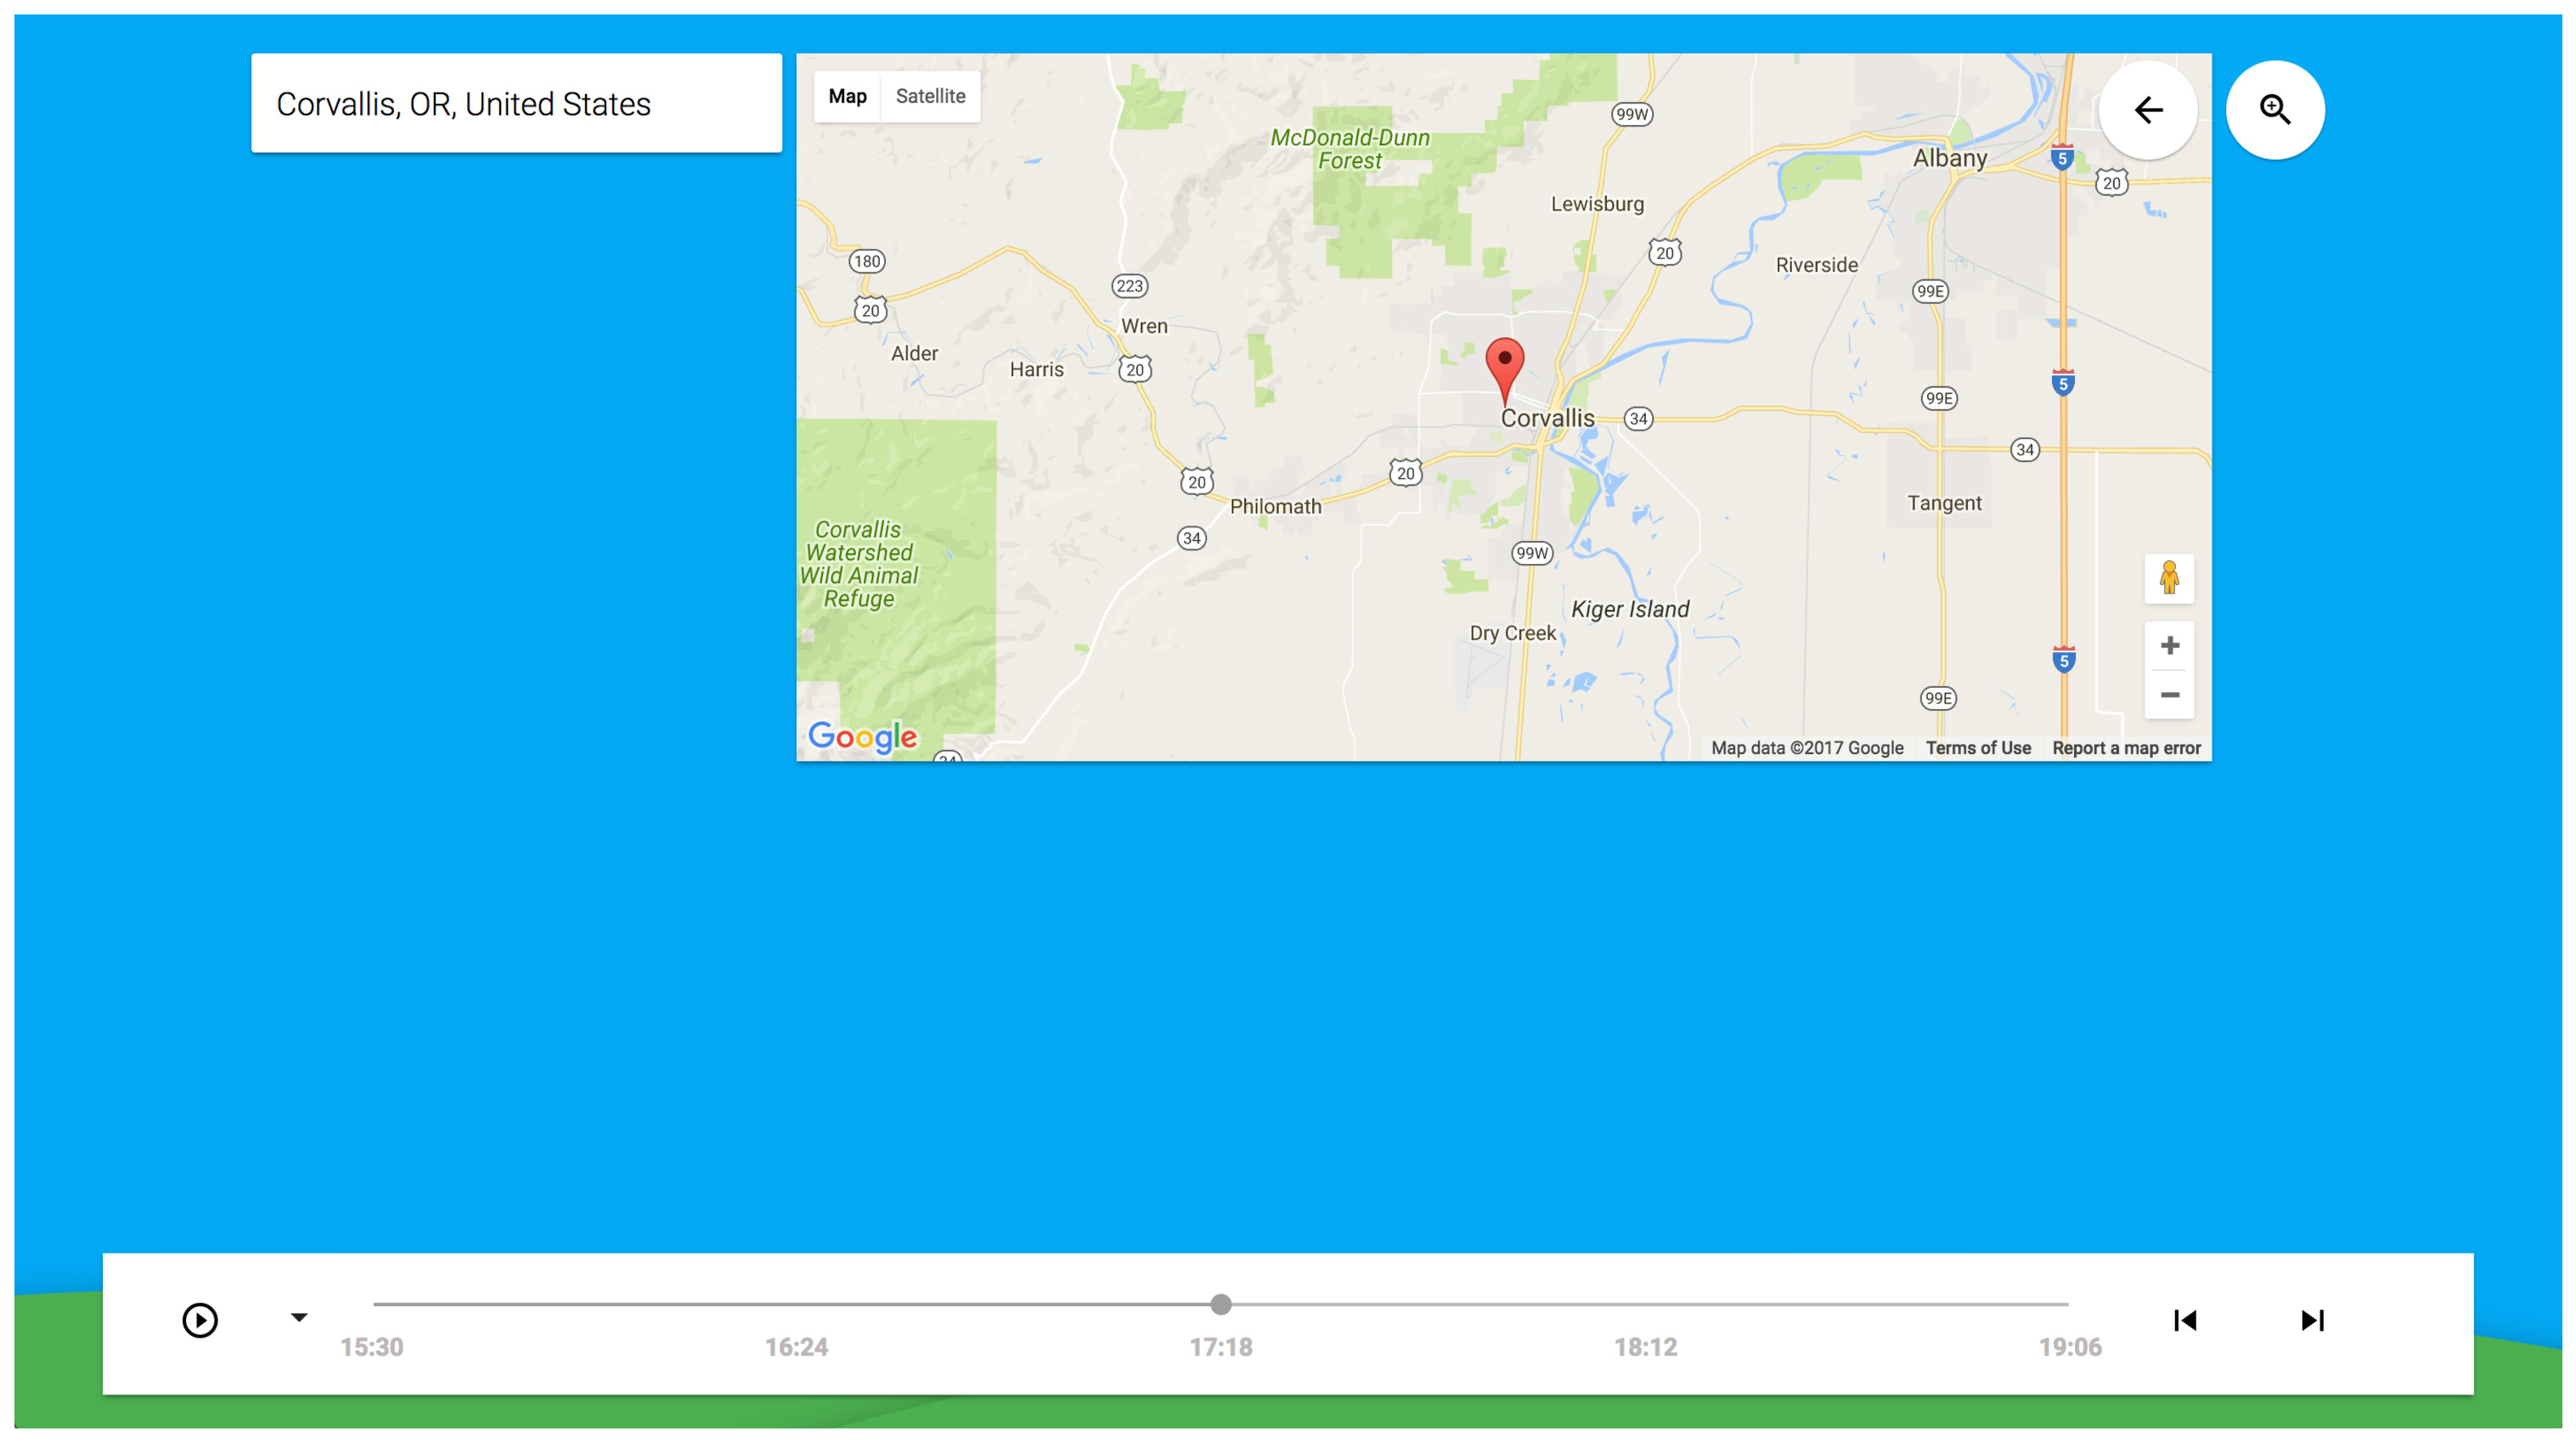
\includegraphics[width=0.8\textwidth]{sim_map.eps}
		\caption{Simulator with map expanded}
	\end{center}
\end{figure}

%%%%%%%%%%%%%%%%%%%%%%%%
%   Weekly Summary     %
%%%%%%%%%%%%%%%%%%%%%%%%
\newpage
\section{Week by Week Summary of Group Activities}

\subsection{Winter Break Week 1}

    \begin{itemize}

    \item Tuned basic simulator UI (non-functional).

	\item Began implementing simulator model using ephemeris JS to perform Sun/Moon
		  position computations. Verified that these computations can be done
		  quickly enough for our purposes.

	\item Built loading screen with simple toggle function. Therefore it requires only
		  one line of code to toggle simulator loading state.

    \end{itemize}

\subsection{Winter Break Week 2}

    \begin{itemize}

    \item Built controller to link simulator model and view.

	\item Made simulator UI "prettier." Added hills to scene.

    \end{itemize}

\subsection{Winter Break Week 3}

    \begin{itemize}

    \item Built reverse geocoding proof of concept using Google Maps.

    \end{itemize}

\subsection{Winter Break Week 4}

    \begin{itemize}

    \item Connected reverse geocoding code to simulator, enabling users to use a search
	      bar to set the simulator to the location of their choice.

    \end{itemize}

\subsection{Week 1}

    \begin{itemize}

	\item Talked to our sponsor about open-sourcing the existing image processor /
		  image processor manager code. He is working on creating an external repo with
		  this code so that we can all (him included) collaborate on it there.

	\item Completed documenting requirements changes from the end of fall term. Got
		  revised requirements document signed by our sponsor.

	\item Implemented basic 2d interpolation code in Python using scipy to see if we
		  would be able to interpolate pre-computed eclipse time values from Nasa.
		  This code did not work for locations off the path of totality.

    \item Added an expanding and collapsing Google Map to the simulator that connects
          to the location search box.

    \item Restricted Google Maps search results to the United States.

    \end{itemize}

\subsection{Week 2}

    \begin{itemize}

    \item Achieved very good (within 1 minute accuracy) results computing eclipse time
		  using 2d interpolation with scipy. This accuracy extends across the United
		  States, both inside and outside the path of totality, including in areas that
		  were previously causing problems, like Florida.

	\item Told our sponsor that this is our big development term, so we are hoping to get
		  working on the image processor / image processor manager components of our
		  project as soon as possible. He is planning to open source these as soon as
		  possible.

    \item Finished integrating Google Map to the simulator. Users can drop markers on the
          map to set their location or use the location search box. Marker drops and search
          results are restricted to the United States.

    \end{itemize}

\subsection{Week 3}

    \begin{itemize}

    \item Altered view rendering of Sun/Moon y position in frame.

	\item Implemented simulator zoom mode.

	\item Met with our sponsor, the Google lead on the Eclipse Megamovie project,
		  Justin Koh, and Gonglue Jiang, a Google UX designer regarding simulator design/
		  feedback.

	\item Updated zoom mode to center Sun in frame following feedback from Justin.

	\item Verified that the reason the simulator looks inaccurate in locations like San
		  Diego (where there is only a partial eclipse) is inaccurate ephemeris JS
		  computations.

	\item Considered/brainstormed various methods for improving ephemeris computations.

    \end{itemize}

\subsection{Week 4}

    \begin{itemize}

    \item Received Gonglue's design mocks from our sponsor.

	\item Proposed solutions to problems raised by the design mocks. See below:

		\begin{itemize}

		\item The hills are quite tall, if left as-is, the Sun/Moon will not become
			  visible until they are at a non-negligible altitude. To solve this,
			  I proposed define 0 degrees of altitude at a point towards the top of the
			  hills. This would mean that the bottom of the hills correspond to an altitude
			  value of less than 0. This should not cause any problems.

		\item The Sun/Moon in the mocks are very large, much more so than in the current
			  simulator, at least in wide mode. If left as-is, this will make the simulator
			  show the eclipse starting much earlier than it is supposed to. To solve this, I
			  proposed that we "stretch" degrees at the altitudes around the Sun. This would
			  potentially enable us to still have a field of view where there are 80 degrees
			  of altitude, but maintain a large Sun/Moon. See an illustration of this concept below:

			  \begin{center}
			  	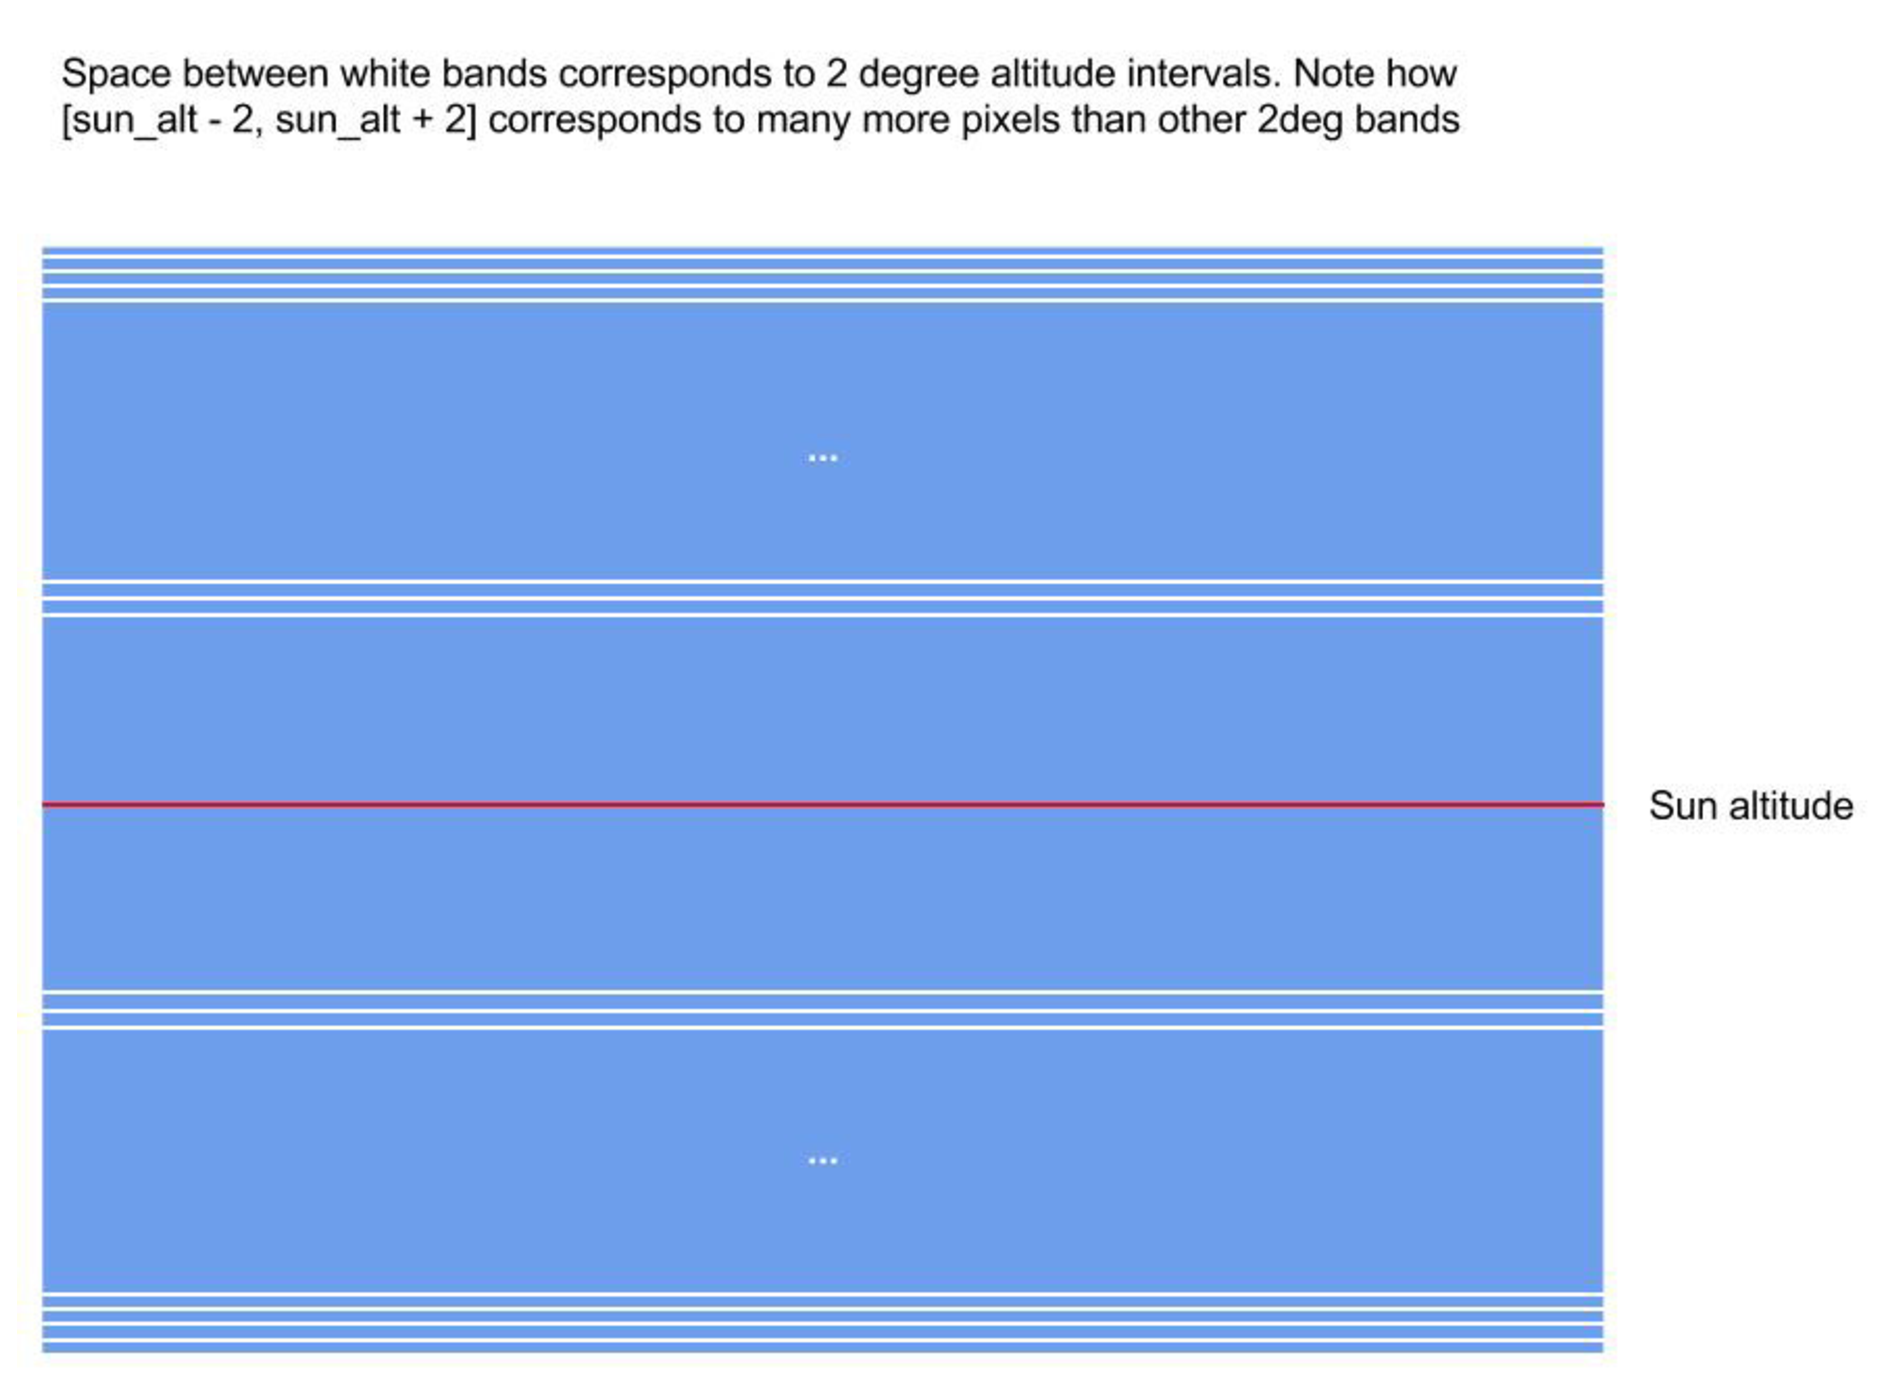
\includegraphics[width=0.6\textwidth]{angle.eps}
			  \end{center}

		\end{itemize}

    \item Added a play button to the simulator that runs through the eclipse from the time the
          the simulator is currently at until the end of the time range. The play function has
          adjustable speed.

    \item Replaced the epehemeris.js library with meuus.js to fix the accuracy issues with Sun and
          Moon position.

    \end{itemize}

\subsection{Week 5}

    \begin{itemize}

    \item Finished the UI tweaks to the top and bottom control bars.

        \begin{itemize}

            \item Centered the location search box and map/zoom buttons.

            \item Changed the map dimensions so it expands to a large rectangle instead of smaller square.

            \item All buttons are now using Material Design Icons instead of text.

            \item Changed color scheme of the control bars to white/grey/black.

            \item Lower control bar floats over the hills instead of sitting at the bottom of the screen.

        \end{itemize}

    \item Asked our sponsor to talk with the Gonglue about getting us useable images of the background
          scene in his mocks of the simulator.

    \end{itemize}

\subsection{Week 6}

    \begin{itemize}

    \item Completed midterm progress report

    \item Met with sponsor, discussed project timeline for the rest of the
          year.

    \end{itemize}

\newpage
\section{Retrospectives}

\begin{table}[!h]
    \centering
    \begin{tabular}{|p{.3\linewidth}|p{.3\linewidth}|p{.3\linewidth}|}

    \cline{3-3}

    \hline \textbf{Positives} & \textbf{Deltas} & \textbf{Actions} \\ \hline

    Completed nearly feature complete alpha release of eclipse simulator &  &  \\ \hline
    Revised (and continue to revise) simulator UI based on sponsor feedback & Current simulator does not sponsor's design mocks & More work/revision required \\ \hline
	Simulator is functional on mobile & Simulator does not work \textit{well} on mobile & Make simulator work well on mobile \\ \hline
     & Image processor development not started & Begin image processor development once sponsor has opportunity to open source the relevant code (end of Feb. 2017) \\ \hline
     & Image processor manager development not started & Begin image processor manager development once sponsor has opportunity to open source the relevant code (end of Feb. 2017) \\ \hline

    \end{tabular}
\end{table}

\end{document}
\00\00\00\00\00\00\00\00\00\00\00\00\00\00\00\00\00\00\00\00\00\00\00\00\00\00\00\00\00
